\documentclass{article}

\usepackage{fullpage}
\usepackage{color}
\usepackage{amsmath}
\usepackage{url}
\usepackage{verbatim}
\usepackage{graphicx}
\usepackage{parskip}
\usepackage{hyperref}
\usepackage{amssymb}
\usepackage{nicefrac}
\usepackage{listings} % For displaying code
\usepackage{algorithm2e} % pseudo-code

% Answers
\def\ans#1{\par\gre{Answer: #1}}
%\def\ans#1{} % Comment this line to produce document with answers

% Colors
\definecolor{blu}{rgb}{0,0,1}
\def\blu#1{{\color{blu}#1}}
\definecolor{gre}{rgb}{0,.5,0}
\def\gre#1{{\color{gre}#1}}
\definecolor{red}{rgb}{1,0,0}
\def\red#1{{\color{red}#1}}
\def\norm#1{\|#1\|}
\let\ask\blu

% Math
\def\R{\mathbb{R}}
\def\argmax{\mathop{\rm arg\,max}}
\def\argmin{\mathop{\rm arg\,min}}
\newcommand{\mat}[1]{\begin{bmatrix}#1\end{bmatrix}}
\newcommand{\alignStar}[1]{\begin{align*}#1\end{align*}}
\def\cond{\; | \;}

% LaTeX
\newcommand{\fig}[2]{\includegraphics[width=#1\textwidth]{#2}}
\newcommand{\centerfig}[2]{\begin{center}\includegraphics[width=#1\textwidth]{#2}\end{center}}
\def\items#1{\begin{itemize}#1\end{itemize}}
\def\enum#1{\begin{enumerate}#1\end{enumerate}}
\newcommand{\matCode}[1]{\lstinputlisting[language=Matlab]{#1.m}}


\begin{document}

\title{CPSC 340 Assignment 2 (due Friday February 3 at 11:55pm)}
\author{}
\date{}
\maketitle
\vspace{-4em}


The assignment instructions are the same as Assignment 1, except you have the option to work in a group of 2.
%If you work in a group, please only hand in \emph{one} assignment.
It is recommended that you work in groups as the assignment is quite long, but please only submit one assignment for the group.

\blu{Name(s) and Student ID(s):}
\ans{\\
Dean Yang 67057695\\
Xuan Tung Luu 30236798
}
\section{Naive Bayes}

In this section we'll implement naive Bayes, a very fast classification method that is often surprisingly accurate for text data with simple representations like bag of words.


\subsection{Naive Bayes by Hand}

Consider the dataset below, which has $12$ training examples and $3$ features:
\[
X = \begin{bmatrix}0 & 1 & 0\\0 & 0 & 1\\0 & 1 & 1\\ 0 & 1 & 1\\ 1 & 1 & 0\\0 & 1 & 0\\0 & 1 & 1\\1 & 0 & 0\\1 & 1 & 0\\1 & 0 & 1\\0 & 1 & 0\\1 & 0 & 0\\\end{bmatrix}, \quad y = \begin{bmatrix}\text{spam}\\\text{spam}\\\text{spam}\\\text{spam}\\\text{spam}\\\text{spam}\\\text{spam}\\\text{not spam}\\\text{not spam}\\\text{not spam}\\\text{not spam}\\\text{not spam}\end{bmatrix}.
\]
The feature in the first column is $<$your name$>$ (whether the e-mail contained your name), in the second column is ``pharmaceutical'' (whether the e-mail contained this word), and the third column is ``PayPal'' (whether the e-mail contained this word).
Suppose you believe that a naive Bayes model would be appropriate for this dataset, and you want to classify the following test example:
\[
\tilde{x} = \begin{bmatrix}1 & 0 & 1\end{bmatrix}.
\]

\pagebreak

\subsubsection{Prior probabilities}

\blu{Compute the estimates of the class prior probabilities} (you don't need to show any work):
\items{
\item$ p(\text{spam})$.
\ans{0.583}
\item $p(\text{not spam})$.
\ans{0.417}
}

\subsubsection{Conditional probabilities}

\blu{Compute the estimates of the 6 conditional probabilities required by naive Bayes for this example}  (you don't need to show any work):
\items{
\item $p(\text{$<$your name$>$} = 1  \cond \text{spam})$.
\ans{$\frac{1}{7}$}
\item $p(\text{pharmaceutical} = 0 \cond \text{spam})$.
\ans{$\frac{1}{7}$}
\item $p(\text{PayPal} = 1  \cond \text{spam})$.
\ans{$\frac{4}{7}$}
\item $p(\text{$<$your name$>$} = 1  \cond \text{not spam})$.
\ans{$\frac{4}{5}$}
\item $p(\text{pharmaceutical} = 0  \cond \text{not spam})$.
\ans{$\frac{3}{5}$}
\item $p(\text{PayPal} = 1  \cond \text{not spam})$.
\ans{$\frac{1}{5}$}
}

\subsubsection{Prediction}


\blu{Under the naive Bayes model and your estimates of the above probabilities, what is the most likely label for the test example? (Show your work.)}
\ans{\\
$P(name=1,pharmaceutical=0,PayPal=1|spam)P(spam)$ 
\\
$=P(name=1|spam)P(pharmaceutical=0|spam)P(PayPal=1|spam)P(spam)$
\\
$=(\frac{1}{7})(\frac{1}{7})(\frac{4}{7})(\frac{7}{12})$
\\
$=\frac{1}{147}$
}
\ans{\\
$P(name=1,pharmaceutical=0,PayPal=1|not spam)P(not spam)$ 
\\
$=P(name=1|not spam)P(pharmaceutical=0|not spam)P(PayPal=1|not spam)P(not spam)$
\\
$=(\frac{4}{5})(\frac{3}{5})(\frac{1}{5})(\frac{5}{12})$
\\
$=\frac{1}{25}$
\\
It is more likely that the test example is not spam.
}


\pagebreak

\subsection{Bag of Words}

  If you run \texttt{python main.py 1.2}, it will load the following dataset:
    \begin{enumerate}
        \item \texttt{X}: A binary matrix. Each row corresponds to a newsgroup post, and each column corresponds to whether a particular word was used in the post. A value of $1$ means that the word occured in the post.
        \item \texttt{wordlist}: The set of words that correspond to each column.
        \item \texttt{y}: A vector with values $0$ through $3$, with the value corresponding to the newsgroup that the post came from.
        \item \texttt{groupnames}: The names of the four newsgroups.
        \item \texttt{Xvalidate} and \texttt{yvalidate}: the word lists and newsgroup labels for additional newsgroup posts.
    \end{enumerate}
    \ask{Answer the following}:
    \begin{enumerate}
        \item Which word corresponds to column 73 of $X$? (This is index 72 in Python.)
        \ans{question}
        \item Which words are present in training example 803 (Python index 802)?
        \ans{'case', 'children', 'health', 'help', 'problem', 'program'}
        \item Which newsgroup name does training example 803 come from?
        \ans{talk.*}
    \end{enumerate}

\pagebreak

\subsection{Naive Bayes Implementation}

   If you run \texttt{python main.py 1.3}
    it will load the newsgroups dataset, fit a basic naive Bayes model and report the validation error.

    The \texttt{predict()} function of the naive Bayes classifier is already implemented.
    However, in \texttt{fit()}
    the calculation of the variable \texttt{p\_xy} is incorrect
    (right now, it just sets all values to $1/2$).
    \ask{Modify this function so that \texttt{p\_xy} correctly
        computes the conditional probabilities of these values based on the
        frequencies in the data set. Submit your code. Report the training and validation errors that you obtain.}
\ans{\\
Naive Bayes training error: 0.200
\\
Naive Bayes validation error: 0.188
}
\begin{center}
      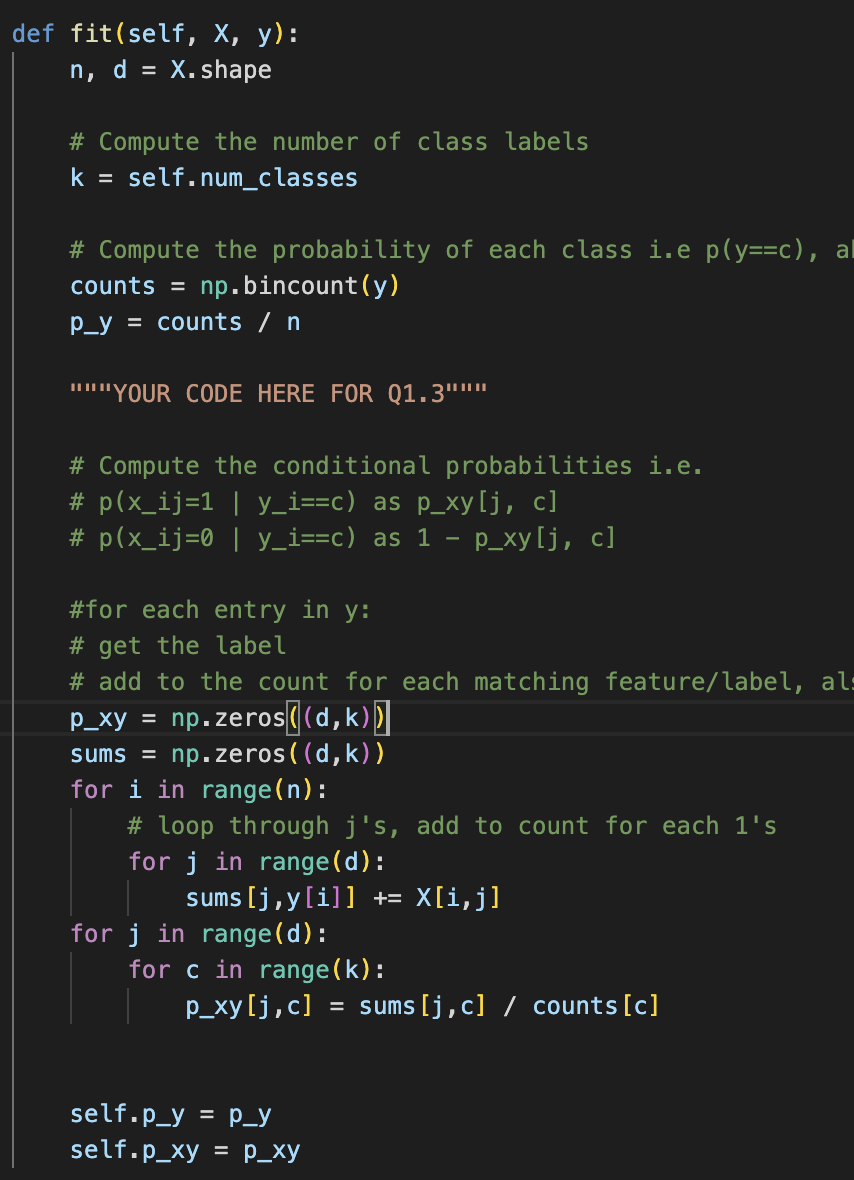
\includegraphics[height=500pt]{1.3.png}
  \end{center}


\pagebreak

\subsection{Runtime of Naive Bayes for Discrete Data}

Assume you have the following setup:
\items{
\item The training set has $n$ objects each with $d$ features.
\item The test set has $t$ objects with $d$ features.
\item Each feature can have up to $c$ discrete values (you can assume $c \leq n$).
\item There are $k$ class labels (you can assume $k \leq n$)
}
You can implement the training phase of a naive Bayes classifier in this setup in $O(nd)$, since you only need to do a constant amount of work for each $X[i,j]$ value. (You do not have to actually implement it in this way for the previous question, but you should think about how this could be done). \blu{What is the cost of classifying $t$ test examples with the model?}

\ans{\\
We have to compute the product between all features in each category. Hence the runtime is $O(tdk)$}
\pagebreak

\section{K-Nearest Neighbours}


In \emph{citiesSmall} dataset, nearby points tend to receive the same class label because they are part of the same state. This indicates that a $k-$nearest neighbours classifier might be a better choice than a decision tree (while naive Bayes would probably work poorly on this dataset). The file \emph{knn.py} has implemented the training function for a $k-$nearest neighbour classifier (which is to just memorize the data) but the predict function always just predicts 1.


\subsection{KNN Prediction}

Fill in the \emph{predict} function in \emph{knn.py} so that the model file implements the k-nearest neighbour prediction rule. You should use Euclidean distance.

Hint: although it is not necessary, you may find it useful to pre-compute all the distances (using the \texttt{utils.euclidean\string_dist\string_squared}) and to use the numpy's \texttt{sort} and/or \texttt{argsort}.
\blu{
\enum{
\item Hand in the predict function.
\\
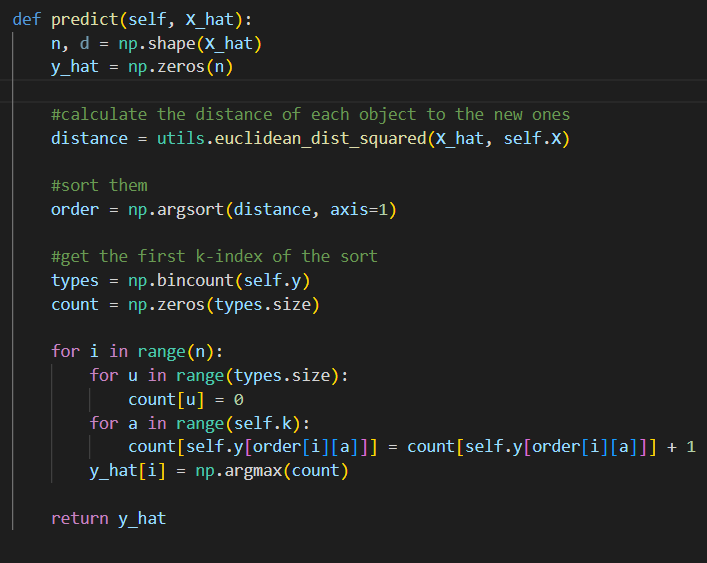
\includegraphics[width=400pt]{2.1.png}
 \\
\item Report  the training and test error obtained on the \emph{citiesSmall} dataset for $k=1$, $k=2$, and $k=3$.
\ans{\\
k:  1
, KNN training error: 0.000
, KNN test error: 0.065
\\
k:  2
, KNN training error: 0.035
, KNN test error: 0.092
\\
k:  3
, KNN training error: 0.028
, KNN test error: 0.066
}
\item Generate a plot with \texttt{utils.plot\_classifier} on the \emph{citiesSmall} dataset (plotting the training points) for $k=1$, using your implementation of kNN. \ask{Include the plot here.} To see if your implementation makes sense, you might want to check against the plot using \texttt{sklearn.neighbors.KNeighborsClassifier}. Remember that the assignment 1 code had examples of plotting with this function and saving the result, if that would be helpful.
\centerfig{.5}{figs/q2.1_knn}
\item If we entered the coordinates of Vancouver into the predict function, would it be predicted to be in a blue state or a red state (for $k=1$)?
\ans{Blue}
\item Why is the training error $0$ for $k=1$?
\ans{Because the data points when we predict will be exactly the same as the data points we fit on (Same X). Therefore, the smallest distance is always 0 and the label is the exact same label as the ones we fit (k=1). As a result, training error = 0.
}
\item If you didn't have an explicit test set, how would you choose $k$?
\ans{We could use cross-validation and try out different k's to pick the k that has the lowest mean error.}
}}

Hint: when writing a function, it is typically a good practice to write one step of the code at a time and check if the code matches the output you expect. You can then proceed to the next step and at each step test is if the function behaves as you expect. You can also use a set of inputs where you know what the output should be in order to help you find any bugs. These are standard programming practices: it is not the job of the TAs or the instructor to find the location of a bug in a long program you've written without verifying the individual parts on their own.

\pagebreak

\subsection{Picking $k$ in KNN}
The file \texttt{data/ccdebt.pkl} contains a subset of \href{https://www23.statcan.gc.ca/imdb/p2SV.pl?Function=getSurvey&SDDS=2620}{Statistics Canada's 2019 Survey of Financial Security}; we're predicting whether a family regularly carries credit card debt, based on a bunch of demographic and financial information about them. (You might imagine social science researchers wanting to do something like this if they don't have debt information available -- or various companies wanting to do it for less altruistic reasons.) If you're curious what the features are, you can look at the \texttt{`feat\_descs'} entry in the dataset dictionary.

Anyway, now that we have our kNN algorithm working,\footnote{If you haven't finished the code for question 2.1, or if you'd just prefer a slightly faster implementation, you can use scikit-learn's \texttt{KNeighborsClassifier} instead. The \texttt{fit} and \texttt{predict} methods are the same; the only difference for our purposes is that \texttt{KNN(k=3)} becomes \texttt{KNeighborsClassifier(n\_neighbors=3)}.} let's try choosing $k$ on this data!

\begin{enumerate}
    \item Remember the bedrock principle: we don't want to look at the test data when we're picking $k$. Inside the \texttt{q2\_2()} function of \texttt{main.py}, implement 10-fold cross-validation, evaluating on the \texttt{ks} set there ($k = \{1, 5, 9, \dots, 29\}$), and store the \emph{mean} accuracy across folds for each $k$ into a variable named \texttt{cv\_accs}.

    Specifically, make sure you test on the first 10\% of the data after training on the remaining 90\%, then test on 10\% to 20\% and train on the remainder, etc -- don't shuffle (so your results are consistent with ours; the data is already in random order). Implement this yourself, don't use scikit-learn or any other existing implementation of splitting. There are lots of ways you could do this, but one reasonably convenient way is to create a \href{https://numpy.org/doc/stable/user/basics.indexing.html#boolean-or-mask-index-arrays}{numpy ``mask'' array}, maybe using \texttt{np.ones(n, dtype=bool)} for an all-\texttt{True} array of length \texttt{n}, and then setting the relevant entries to \texttt{False}. It also might be helpful to know that \texttt{\textasciitilde ary} flips a boolean array (\texttt{True} to \texttt{False} and vice-versa).

    \blu{Submit this code}, following the general submission instructions to include your code in your results file.
\begin{center}
    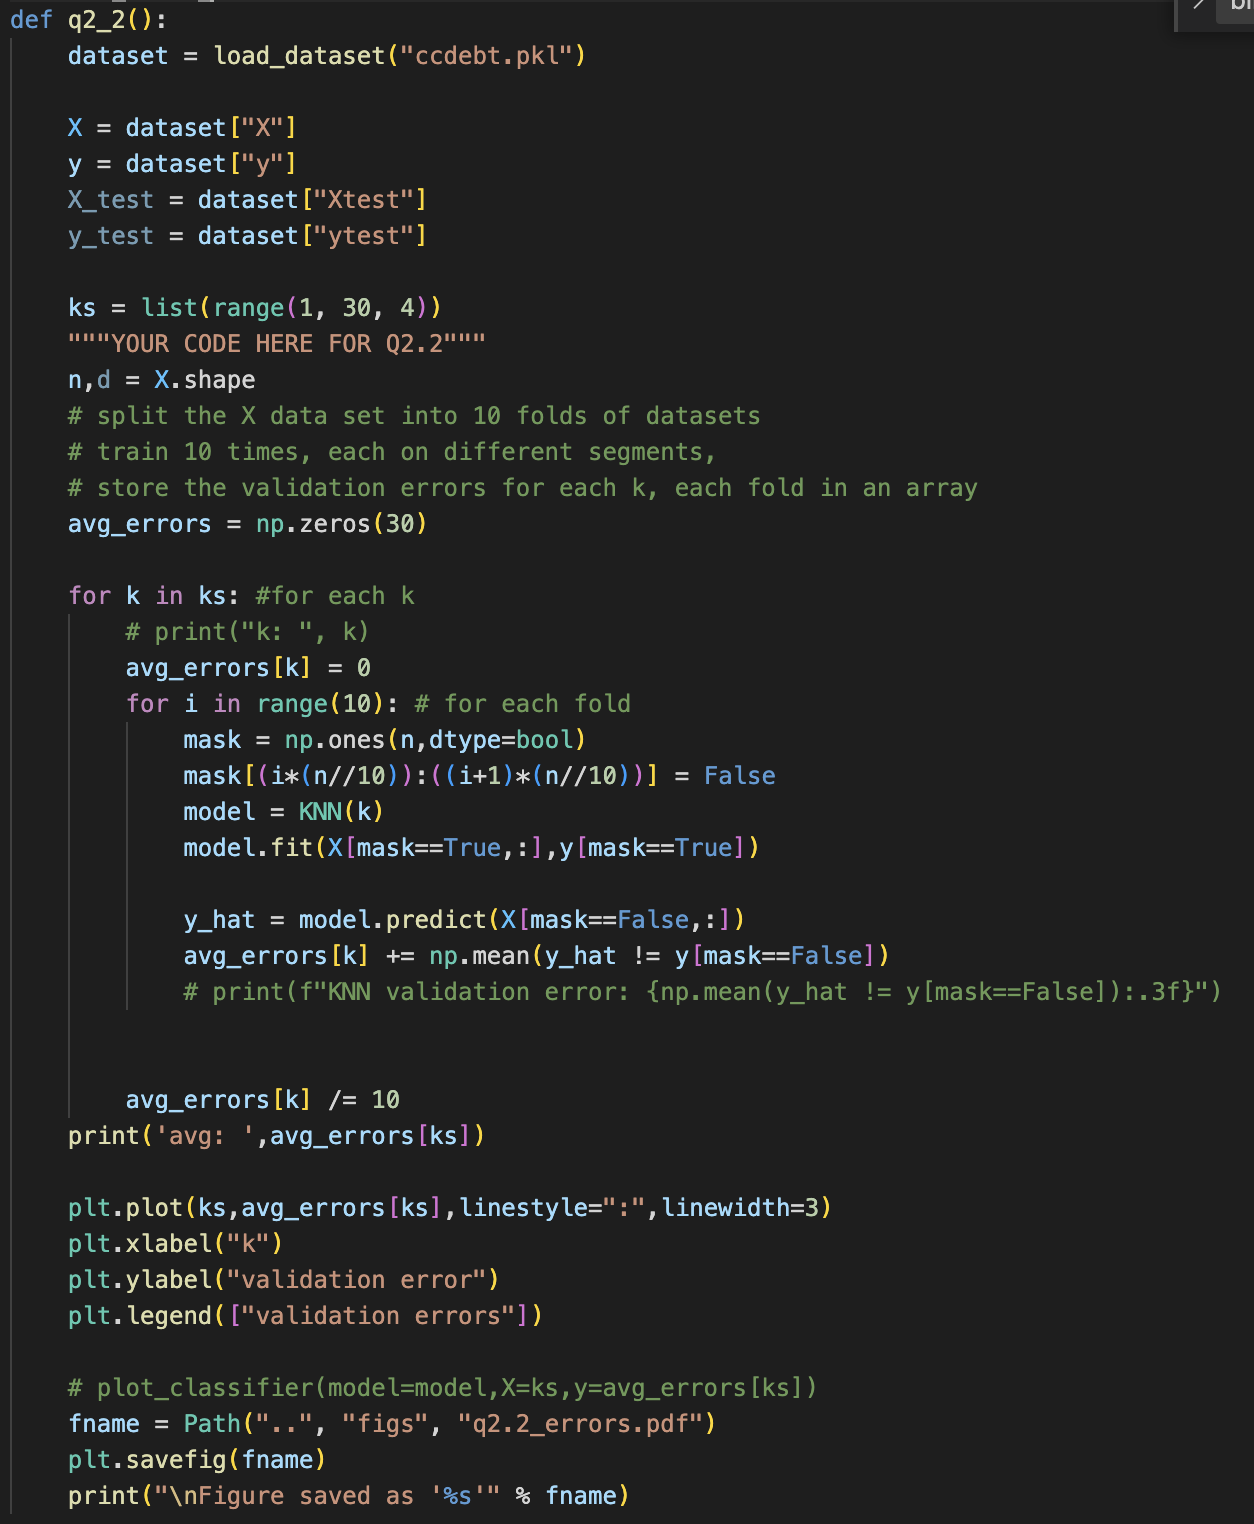
\includegraphics[height=500pt]{2.2.png}
\end{center}
    \item The point of cross-validation is to get a sense of what the test error for a particular value of $k$ would be. Implement a loop to compute the test accuracy for each value of $k$ above. \ask{Submit a plot of the cross-validation and test accuracies as a function of $k$.} Make sure your plot has axis labels and a legend.
    \centerfig{.5}{figs/q2.2_errors}
    \item Which $k$ would cross-validation choose in this case? Which $k$ has the best test accuracy? Would the cross-validation $k$ do okay (qualitatively) in terms of test accuracy?
    \ans{Cross-validation should choose k=17. k=9 has the best test accuracy. Both the validation set and test set produced very similar error rates. Although k=9 has the best test accuracy, k=17 would do okay since the difference is less than 0.01}
    \item Separately, \ask{submit a plot of the training error as a function of $k$. How would the $k$ with best training error do in terms of test error, qualitatively?}
    \ans{\\
    No, it is not an accurate representation of the test error as training error will overfit with itself at lower k. k=1 performs the best for the training set but has the highest error rate for the test set.}
    \centerfig{.5}{figs/q2.2_trainingerrors}
    
\end{enumerate}

\pagebreak

\section{Random Forests}


 \subsection{Implementation}

The file \texttt{vowels.pkl} contains a supervised learning dataset where we are trying to predict which of the 11 ``steady-state'' English vowels that a speaker is trying to pronounce.

You are provided with a \texttt{RandomStump} class that differs from
\texttt{DecisionStumpInfoGain} in that
it only considers $\lfloor \sqrt{d} \rfloor$ randomly-chosen features.\footnote{The notation $\lfloor x\rfloor$ means the ``floor'' of $x$, or ``$x$ rounded down''. You can compute this with \texttt{np.floor(x)} or \texttt{math.floor(x)}.}
You are also provided with a \texttt{RandomTree} class that is exactly the same as
\texttt{DecisionTree} except that it uses \texttt{RandomStump} instead of
\texttt{DecisionStump} and it takes a bootstrap sample of the data before fitting.
In other words, \texttt{RandomTree} is the entity we discussed in class, which
makes up a random forest.

If you run \texttt{python main.py 3} it will fit a deep \texttt{DecisionTree}
using the information gain splitting criterion. You will notice that the model overfits badly.

   \begin{enumerate}
        \item Using the provided code, evaluate the \texttt{RandomTree} model of unlimited depth. \ask{Why doesn't the random tree model have a training error of 0?}
        \ans{Because for random trees, they are only trained on a bootstrapped subset of datapoints. The training error may not be zero as the individual trees do not have the complete picture of the dataset, even at infinite depth.}
        \item For \texttt{RandomTree}, if you set the \texttt{max\_depth} value to \texttt{np.inf}, \ask{why do the training functions terminate instead of making an infinite number of splitting rules?}
        \ans{When the splitting function reaches the state where there is zero infogain available within any of the split (i.e. all labels are the same within each split), the function will terminate, as there is no more data to split. We know that this state can always be reached, as we do not have infinite data to split.}
        \item Complete the \texttt{RandomForest} class in \texttt{random\string_tree.py}. This class takes in hyperparameters \texttt{num\string_trees} and \texttt{max\string_depth} and
        fits \texttt{num\string_trees} random trees each with maximum depth \texttt{max\string_depth}. For prediction, have all trees predict and then take the mode. \ask{Submit this code.} 
        \begin{center}
            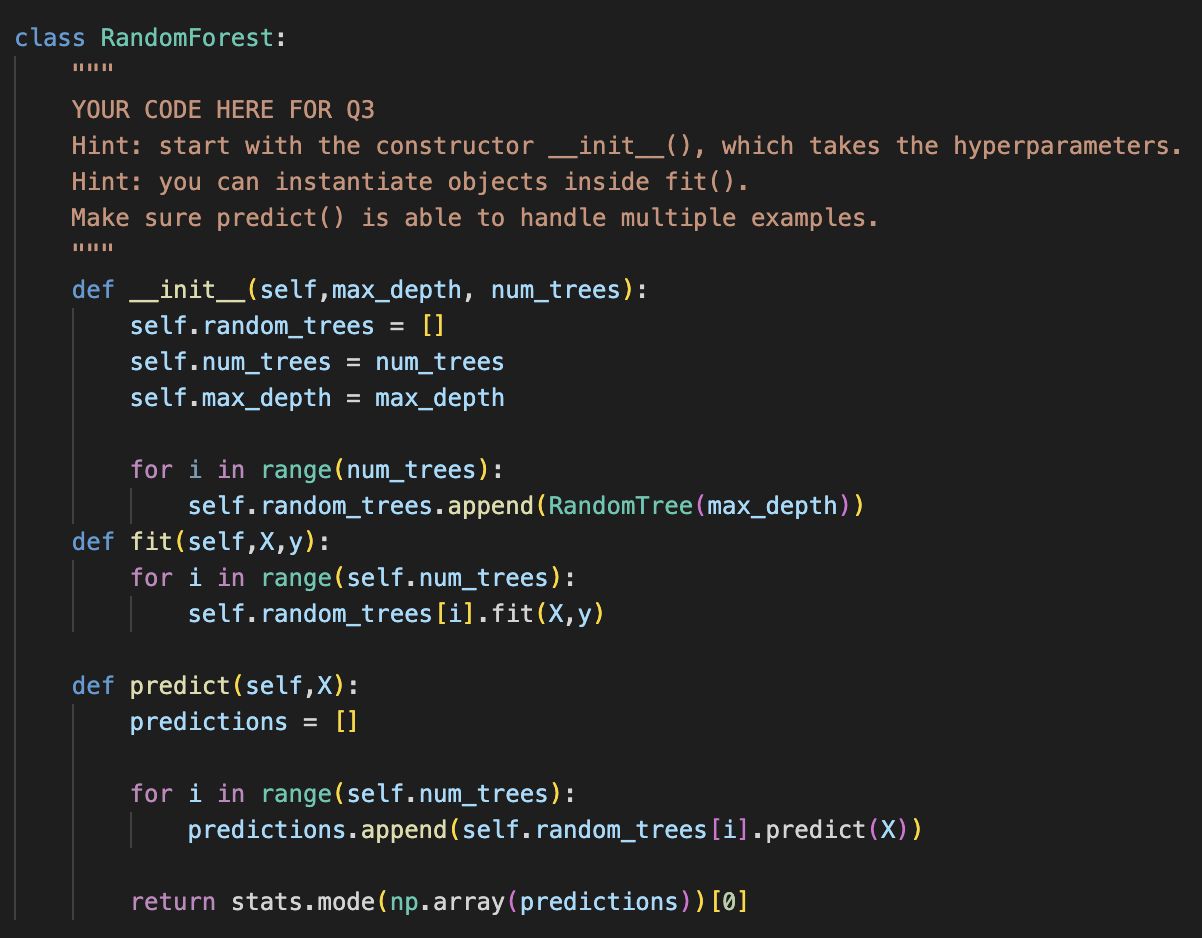
\includegraphics[width=400pt]{3.3.png}
        \end{center}
        \item Using 50 trees, and a max depth of $\infty$, \ask{report the training and testing error}. Compare this to what we got with a single \texttt{DecisionTree} and with a single \texttt{RandomTree}. \ask{Are the results what you expected? Discuss.}
        \ans{\\
        Random Forest: Training error: 0.000, Testing error: 0.167\\
        Decision Tree: Training error: 0.000, Testing error: 0.367\\
        Random Tree: Training error: 0.174, Testing error: 0.545\\
        Random forest performs the best in the testing error. This is because it takes the mode of many random trees, which tend to create a label that is more likely to be correct. It also has a training error of 0, similar to the Decision Tree. Explanation below.
        }
        \item \ask{Why does a random forest typically have a training error of 0, even though random trees typically have a training error greater than 0?}
        \ans{\\
        After creating a forest of 50 random trees, it is highly likely that the individual biases of bootstrap samples (and hence the random trees) average out to give us a 
        an accurate representation of the entire training dataset, which is why the training error is 0.
        }
    \end{enumerate}

\pagebreak

\section{K-Means Clustering}

If you run \verb|python main.py 4|, it will load a dataset with two features
and a very obvious clustering structure. It will then apply the $k$-means algorithm
with a random initialization. The result of applying the
algorithm will thus depend on the randomization, but a typical run might look like this:
\centerfig{.5}{figs/kmeans_basic.png}
(Note that the colours are arbitrary due to the label switching problem.)
But the `correct' clustering (that was used to make the data) is something more like this:
\centerfig{.5}{figs/kmeans_good.png}

\pagebreak

\subsection{Selecting among k-means Initializations}

If you run the demo several times, it will find different clusterings. To select among clusterings for a \emph{fixed} value of $k$, one strategy is to minimize the sum of squared distances between examples $x_i$ and their means $w_{y_i}$,
\[
f(w_1,w_2,\dots,w_k,y_1,y_2,\dots,y_n) = \sum_{i=1}^n \norm{x_i - w_{y_i}}_2^2 = \sum_{i=1}^n \sum_{j=1}^d (x_{ij} - w_{y_ij})^2.
\]
 where $y_i$ is the index of the closest mean to $x_i$. This is a natural criterion because the steps of k-means alternately optimize this objective function in terms of the $w_c$ and the $y_i$ values.

 \blu{\enum{
 \item In the \texttt{kmeans.py} file, complete the \texttt{error()} method. \texttt{error()} takes as input the data used in fit (\texttt{X}), the indices of each examples' nearest mean (\texttt{y}), and the current value of means (\texttt{means}). It returns the value of this above objective function. Hand in your code.
 \begin{center}
     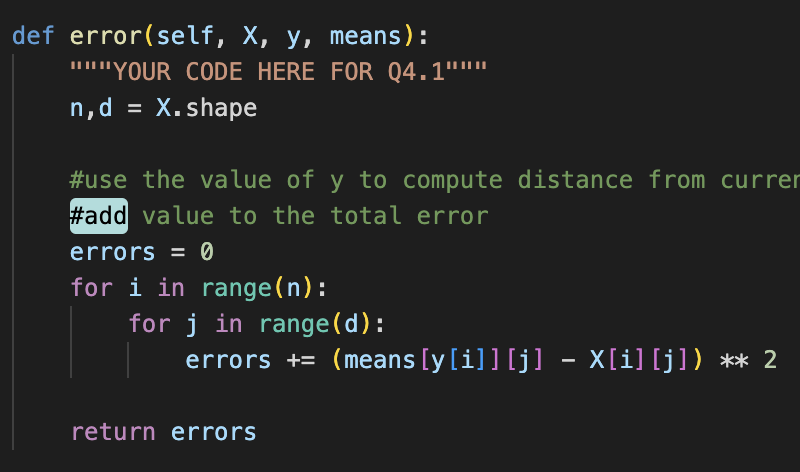
\includegraphics[width=400pt]{4.1.1.png}
 \end{center}
 \item Instead of printing the number of labels that change on each iteration, what trend do you observe if you print the value of this error after each iteration of the k-means algorithm?
 \ans{It decreases from start to finish in a non-linear fashion. In some runs, the value will decrease by a lot in one iteration, which may be due to means crossing clusters.} 
 \item Run $k$-means 50 times (with $k=4$) and take the one with the lowest error. \ask{Report the lowest error obtained.} Visualize the clustering obtained by this model, and \ask{submit your plot}.
 \ans{The lowest error obtained: 3071.4680526538564}
    \begin{center}
        \centerfig{.5}{figs/kmeans_lowest_error}
    \end{center}
 }}


 \pagebreak

 \subsection{Selecting $k$ in k-means}

 We now turn to the task of choosing the number of clusters $k$.

 \blu{\enum{
 \item Explain why the error function should not be used to choose $k$.
 \ans{If we choose k so that error is minimized, it will always select k=n clusters as each data point will have its own cluster, which results in error of 0. This is not useful.}
 \item Explain why even evaluating the error function on test data still wouldn't be a suitable approach to choosing $k$.
 \ans{The test data should not affect how we train our model in any way (bedrock principle), or we may overfit to the test data.}
 \item Hand in a plot of the minimum error found across 50 random initializations, as you vary $k$ from $1$ to $10$.
 \begin{center}
     \centerfig{.7}{figs/kmeans_lowesterrors.pdf}
 \end{center}
 \item The \emph{elbow method} for choosing $k$ consists of looking at the above plot and visually trying to choose the $k$ that makes the sharpest ``elbow" (the biggest change in slope). What values of $k$ might be reasonable according to this method? Note: there is not a single correct answer here; it is somewhat open to interpretation and there is a range of reasonable answers.
 }}
 \ans{\\
    The plot has the sharpest bend at k=3, another reasonable answer is k=4. This is a pretty reasonable method considering that the top two clusters are much more closely grouped than the other two, so it is reasonable to consider them as 1 cluster.
 }
 

 \pagebreak

 \subsection{$k$-Medians}

 The data in \emph{clusterData2.pkl} is the exact same as the above data, except it has 4 outliers that are very far away from the data.

 \blu{\enum{
 \item Visualize the clustering obtained by running k-means 50 times (with $k=4$) on \emph{clusterData2.pkl} and taking the one with the lowest error. Are you satisfied with the result?
 \ans{No, the datapoints on the corners of the graph are classified as in the same clusters as the center ones, even though they are clearly in different clusters.}
 \item Hand in the elbow plot for this data. What values of $k$ might be chosen by the elbow method for this dataset?
 \ans{k=8 has a large change in slope.}
\centerfig{.7}{figs/kmeans4.3.2_lowesterrors}
 \item Instead of the squared distances between the examples $x_i$ and their cluster centers, consider measuring the distance to the cluster centers in the L1-norm,
\[
f(w_1,w_2,\dots,w_k,y_1,y_2,\dots,y_n) = \sum_{i=1}^n \norm{x_i - w_{y_i}}_1 = \sum_{i=1}^n \sum_{j=1}^d |x_{ij} - w_{y_ij}|.
\]
Hand in the elbow plot for k-means when we measure the error of the final model with the L1-norm.
What value of $k$ would be chosen by the elbow method?
 \ans{k=3 has the largest change in slope}
\centerfig{.7}{figs/kmeans4.3.3_lowesterrors}
 \item The k-means algorithm tries to minimize the squared error and not the L1-norm error, so in the last question there is a mis-match between what the learning algorithm tries to minimize and how we measure the final error. We can try to directly minimize the L1-norm with the $k$-\emph{medians} algorithm, which assigns examples to the nearest $w_c$ in the L1-norm and to update the $w_c$ by setting them to the ``median" of the points assigned to the cluster (we define the $d$-dimensional median as the concatenation of the median of the points along each dimension). Implement the $k$-medians algorithm, and hand in your code and the the plot obtained by minimizing the L1-norm error across 50 random initializations of $k$-medians with $k=4$.
 \begin{center}
 \end{center}
 \begin{center}
     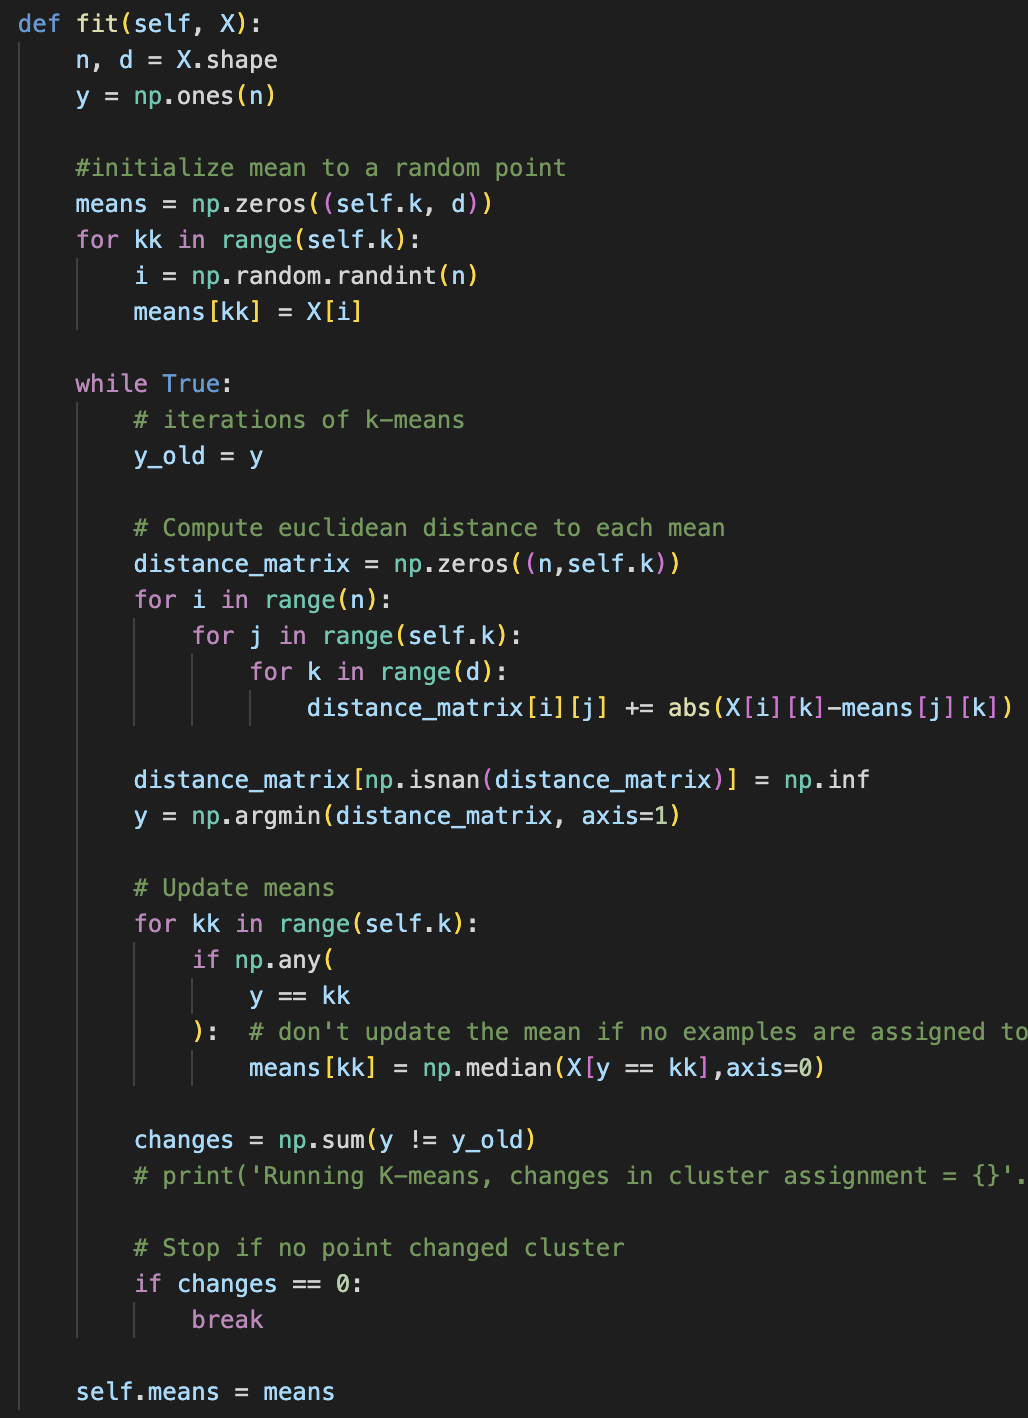
\includegraphics[width=400pt]{figs/4.3.4.png}
 \end{center}
 \begin{center}
     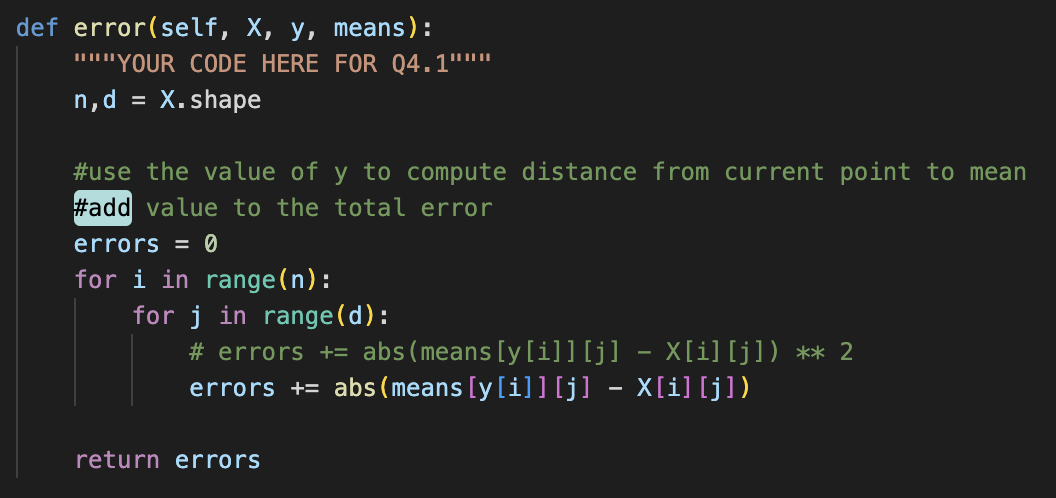
\includegraphics[width=400pt]{figs/4.3.4.2.png}
 \end{center}
  \begin{center}
     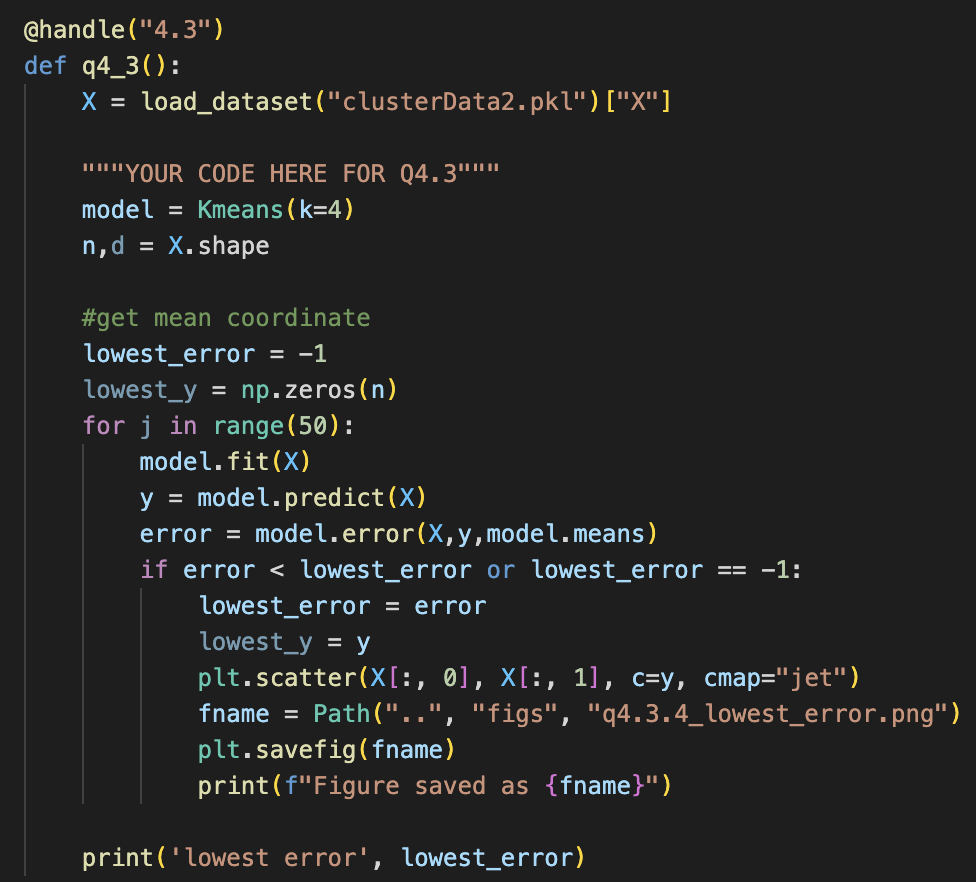
\includegraphics[width=400pt]{figs/4.3.4.3.png}
 \end{center}
 \begin{center}
     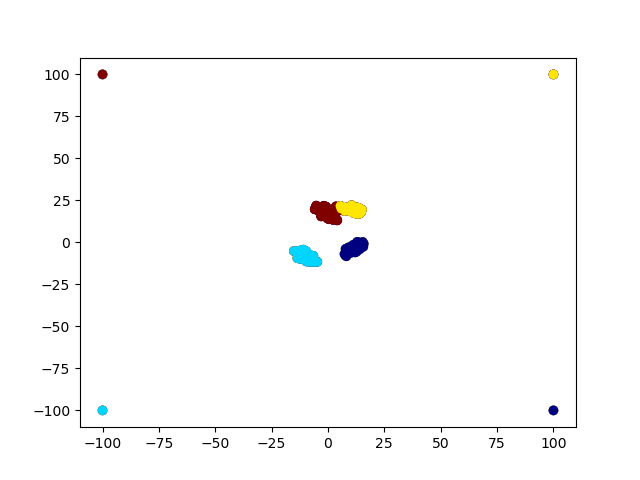
\includegraphics[width=400pt]{figs/q4.3.4_lowest_error.png}
 \end{center}
}
}
\pagebreak

\section{Very-Short Answer Questions}

\blu{Write a short one or two sentence answer to each of the questions below}. Make sure your answer is clear and concise.

\enum{
 \item What is a feature transformation that you might do to address a ``coupon collecting'' problem in your data?
 \ans{We can aggregate the features - group features into larger categories. }
\item What is one reason we would want to look at scatterplots of the data before doing supervised learning?
\ans{Makes sure that we properly check the data for outliers.}
 \item When we fit decision stumps, why do we only consider $>$ (for example) and not consider $<$ or $\geq$?
 \ans{It is possible to use one of the other two comparisons for our stump, as they perform similar functions in splitting our data into two groups, but is it pointless to use multiple of them at once as we need a unified method for splitting data so our result is consistent.}
\item What is a reason that the data may not be IID in the email spam filtering example from lecture?
\ans{Words in emails are written in phrases, so they are not completely independent of each other.}
\item What is the difference between a validation set and a test set?
\ans{Validation set is split from the training data which we can use to choose our hyper-parameters to optimize our model. Test set is only evaluated after everything is finalized, and cannot interfere with our model in any way or it will violate the bedrock principle.}
\item Why can't we (typically) use the training error to select a hyper-parameter?
\ans{Choosing our hyper-parameter to minimize our training error will typically result in overfitting to the training dataset.}
\item If you can fit one model in $10$ sec., how long (in days) does it take to find the best among a set of $16$ hyperparameter values using leave-one-out cross-validation on a dataset containing $n=4320$ examples?
\ans{$4320*16*10s$= 8 days}
\item{Na{\"i}ve Bayes makes the assumption that all features are conditionally independent given the class label. Why is this assumption necessary and what would happen without it?}
\ans{It is necessary because we do not have infinite data to work with. Without it there would not be enough data to generate probabilities for emails that have not been encountered before.}
\item Why is KNN considered a non-parametric method and what are two undesirable consequences of KNNs non-parametric design?
\ans{KNN is considered a non-parametric method because the KNN model's number of parameters grows with n. KNNs may be undesirable because the runtime for classifying a single test example is $O(nd)$, and we also require $O(nd)$ to store the training dataset.}
\item For any parametric model, how does increasing number of training examples $n$ affect the two parts of the fundamental trade-off.
\ans{Increasing $n$ may cause approximation error to decrease, but training error should remain at similar values.}
\item Suppose we want to classify whether segments of raw audio represent words or not. What is an easy way to make our classifier invariant to small translations of the raw audio?
\ans{We can augment our data by producing many duplicates of the same audio but with small translations.}
\item Both supervised learning and clustering models take in an input $x_i$ and produce a label $y_i$. What is the key difference?
\ans{Clustering models do not have an associated label beforehand. Supervised learning can use the $y_i$ label to evaluate our results. Clustering models rely on human interpretation.}
\item In $k$-means clustering the clusters are guaranteed to be convex regions. Are the areas that are given the same label by KNN also convex?
}
\ans{No, it entirely depends on the locations of datapoints.}

\end{document}
